\documentclass[../main.tex]{subfiles}

\begin{document}

\problem{1}

\problempart{a} 
Derive the Hugoniot Eqution.

\assumptions{}
1-D, steady flow.
Inviscid.
Calorically perfect gas (constant specific heats).
Uniform pressure distribution around the CV.
No heat addition (adiabatic).
No work done on or by the CV.

\solution{}

Beginning with the 1-D continuity equation and expressing both velocities in terms of the densities and the other velocity:

\[
    \rho_1 u_1 = \rho_2 u_2
\]

\[
    u_1 = u_2 \left({\frac{\rho_2}{\rho_1}}\right)
\]

\[
    u_2 = u_1 \left({\frac{\rho_1}{\rho_2}}\right)
\]

The 1-D momentum equation:

\[
    p_1 + \rho_1 u_1^2 = p_2 + \rho_2 u_2^2    
\]

Plugging in velocities in terms of 1-D continuity and rearranging:

\[
    p_1 + \rho_1 u_1^2 = p_2 + \rho_2 \left[{u_1 \left({\frac{\rho_1}{\rho_2}}\right)}\right]^2
\]

\[
    (p_1-p_2) =  u_1^2 \left[{\rho_2 \left({\frac{\rho_1}{\rho_2}}\right)^2 - \rho_1}\right]
\]

\[
    (p_1-p_2) = u_1^2 \left[{\left({\frac{\rho_1^2}{\rho_2}}\right) - \rho_1}\right]
\]

\[
    (p_1-p_2) = u_1^2 \left({\frac{\rho_1}{\rho_2}}\right) \left({\rho_1-\rho_2}\right)
\]

We now have relationships for \(u_1\) and \(u_2\) in terms of pressures and densities.

\[
    u_1^2 = \left({\frac{p_1-p_2}{\rho_1-\rho_2}}\right) \left({\frac{\rho_2}{\rho_1}}\right)
\]

\[
    u_2^2 = \left({\frac{p_2-p_1}{\rho_2-\rho_1}}\right) \left({\frac{\rho_1}{\rho_2}}\right)
\]

Next, the 1-D energy equation (adiabatic, no work):

\[
    h_1 + \frac{u_1^2}{2} = h_2 + \frac{u_2^2}{2} 
\]    

The definition of enthalpy, \(h\).

\[
    h = e + \frac{p}{\rho}    
\]

Recasting the 1-D energy equation with the definition of enthalpy and rearranging:

\[
    e_1 + \frac{p_1}{\rho_1} + \frac{u_1^2}{2} = e_2 + \frac{p_2}{\rho_2} + \frac{u_2^2}{2} 
\] 

\[
    e_1 + \frac{p_1}{\rho_1} + \frac{1}{2} \left[{\left({\frac{p_1-p_2}{\rho_1-\rho_2}}\right) \left({\frac{\rho_2}{\rho_1}}\right)}\right] =\
    e_2 + \frac{p_2}{\rho_2} + \frac{1}{2} \left[{\left({\frac{p_2-p_1}{\rho_2-\rho_1}}\right) \left({\frac{\rho_1}{\rho_2}}\right)}\right]
\] 


\[
   0  =  \left({e_2 - e_1}\right) + \left({\frac{p_2}{\rho_2}-\frac{p_1}{\rho_1}}\right) + 
   \frac{1}{2} \left[{\left({\frac{p_2-p_1}{\rho_2-\rho_1}}\right) \left({\frac{\rho_1}{\rho_2} - \frac{\rho_2}{\rho_1}}\right)}\right]
\]

\[
   0  =  \left({e_2 - e_1}\right) + \left({\frac{p_2\rho_1 - p_1\rho_2}{\rho_1\rho_2}}\right) + 
   \frac{1}{2} \left[{\left({\frac{p_2-p_1}{\rho_2-\rho_1}}\right) \left({\frac{\rho_1^2-\rho_2^2}{\rho_1\rho_2}}\right)}\right]
\]

\[
   0  =  \left({e_2 - e_1}\right) + 
   \left({\frac{1}{\rho_1\rho_2}}\right)
   \left[{
    \left({p_2\rho_1 - p_1\rho_2}\right) +
    \frac{1}{2} \left({\frac{p_2-p_1}{\rho_2-\rho_1}}\right) \left({\rho_1^2-\rho_2^2}\right)
   }\right]
\]

\[
    0  =  \left({e_2 - e_1}\right) + 
    \left({\frac{1}{\rho_1\rho_2}}\right)
    \left[{
    \left({p_2\rho_1 - p_1\rho_2}\right) +
    \frac{1}{2} \left({\frac{p_1-p_2}{\rho_1-\rho_2}}\right) \left({\rho_1-\rho_2}\right) \left({\rho_1+\rho_2}\right)
    }\right]
\]

\[
    0  =  \left({e_2 - e_1}\right) + 
    \left({\frac{1}{\rho_1\rho_2}}\right)
    \left[{
    \left({p_2\rho_1 - p_1\rho_2}\right) +
    \frac{1}{2} \left({p_1-p_2}\right) \left({\rho_1+\rho_2}\right)
    }\right]
\]

\[
    0  =  \left({e_2 - e_1}\right) + 
    \left({\frac{1}{\rho_1\rho_2}}\right)
    \left[{
    \left({p_2\rho_1 - p_1\rho_2}\right) +
    \frac{1}{2} \left({p_1\rho_1 + p_1\rho_2 - p_2\rho_1 -p_2\rho_2}\right)
    }\right]
\]

\[
    0  =  \left({e_2 - e_1}\right) + 
    \left({\frac{1}{2}}\right)
    \left({\frac{1}{\rho_1\rho_2}}\right)
    \left({p_1\rho_1 - p_1\rho_2 + p_2\rho_1 -p_2\rho_2}\right)
\]

\[
    \left({e_2 - e_1}\right) =
    \left({\frac{1}{2}}\right)
    \left({\frac{p_1}{\rho_2} - \frac{p_1}{\rho_1} + \frac{p_2}{\rho_2} - \frac{p_2}{\rho_1}}\right)
\]

\[
    \left({e_2 - e_1}\right) =
    \left({\frac{p_1 + p_2}{2}}\right)
    \left({\frac{1}{\rho_1} - \frac{1}{\rho_2}}\right)
\]

We now have one of the common forms of the Hugoniot Equation:

\[
    \left({e_2 - e_1}\right) =
    \left({\frac{p_1 + p_2}{2}}\right)
    \left({\nu_1 - \nu_2}\right)
\]

For a CPG, internal energy, \(e\):

\[
    e = c_\nu T
\]   

Substituting the above relationship into our initial Hugoniot Equation:

\[
    c_\nu \left({T_2 - T_1}\right) =
    \left({\frac{p_1 + p_2}{2}}\right)
    \left({\nu_1 - \nu_2}\right)
\]

For a CPG, \(c_\nu\):

\[
    c_\nu = \frac{R}{\gamma-1}
\] 

Substituting and rearranging:

\[
    \frac{R}{\gamma-1} \left({T_2 - T_1}\right) =
    \left({\frac{p_1 + p_2}{2}}\right)
    \left({\nu_1 - \nu_2}\right)
\]

The ideal gas equation of state:

\[
    T = \frac{p \nu}{R}
\]    

Substituting and rearranging to solve for \(p_2/p_1\):

\[
    \frac{R}{\gamma-1} \left({\frac{p_2 \nu_2}{R} - \frac{p_1 \nu_1}{R}}\right) =
    \left({\frac{p_1 + p_2}{2}}\right)
    \left({\nu_1 - \nu_2}\right)
\]

\[
    \frac{2}{\gamma-1} \left({p_2 \nu_2 - p_1 \nu_1}\right) =
    \left({p_1 + p_2}\right)
    \left({\nu_1 - \nu_2}\right)
\]

\[
    \frac{2}{\gamma-1} \left({p_2 \nu_2 - p_1 \nu_1}\right) =
    p_1 \nu_1 - p_1 \nu_2 + p_2 \nu_1 - p_2 \nu_2
\]

\[
    \left({\frac{2}{\gamma-1} + 1}\right) \left({p_2 \nu_2 - p_1 \nu_1}\right) =
    \left({p_2 \nu_1 - p_1 \nu_2}\right)
\]

\[
    \left({\frac{\gamma+1}{\gamma-1}}\right)  =
    \frac{\left({p_2 \nu_1 - p_1 \nu_2}\right)}
    {\left({p_2 \nu_2 - p_1 \nu_1}\right)}
\]

\[
    \left({\frac{\gamma+1}{\gamma-1}}\right)  =
    \frac{\left({\frac{p_2}{p_1} \nu_1 - \nu_2}\right)}
    {\left({\frac{p_2}{p_1} \nu_2 - \nu_1}\right)}
\]

\[
    \left({\frac{\gamma+1}{\gamma-1}}\right) {\left({\frac{p_2}{p_1} \nu_2 - \nu_1}\right)}  =
    \left({\frac{p_2}{p_1} \nu_1 - \nu_2}\right)
\]

\[
    \left({\frac{\gamma+1}{\gamma-1}}\right) {\left({\frac{p_2}{p_1} \nu_2 - \nu_1}\right)}  =
    \left({\frac{p_2}{p_1} \nu_1 - \nu_2}\right)
\]

\[
    \frac{p_2}{p_1} \left[{\left({\frac{\gamma+1}{\gamma-1}}\right) \nu_2 - \nu_1 }\right] =
    \left({\frac{\gamma+1}{\gamma-1}}\right) \nu_1 - \nu_2
\]

\[
    \frac{p_2}{p_1} = \left[{
        \frac{\left({\frac{\gamma+1}{\gamma-1}}\right) \nu_1 - \nu_2}{{\left({\frac{\gamma+1}{\gamma-1}}\right) \nu_2 - \nu_1 }}
    }\right]
\]

\[
    \frac{p_2}{p_1} = \left[{
        \frac{\left({\frac{\gamma+1}{\gamma-1}}\right) \frac{\nu_1}{\nu_2} - 1}{{\left({\frac{\gamma+1}{\gamma-1}}\right) - \frac{\nu_1}{\nu_2} }}
    }\right]
\]

The relation between density, \(\rho\), and specific volume, \(\nu\):

\[
    \rho = \frac{1}{\nu}
\]

Substituting the above relation yields the final form of the Hugoniot Equation:

\[
    \boxed{
    \frac{p_2}{p_1} = \left[{
        \frac{\left({\frac{\gamma+1}{\gamma-1}}\right) \frac{\rho_2}{\rho_1} - 1}{{\left({\frac{\gamma+1}{\gamma-1}}\right) - \frac{\rho_2}{\rho_1} }}
    }\right]
    }
\]

\discussion{}

\problempart{b}

\solution{}

\[
    \frac{p_2}{p_1} = \left[{
        \frac{\left({\frac{\gamma+1}{\gamma-1}}\right) \frac{\rho_2}{\rho_1} - 1}{{\left({\frac{\gamma+1}{\gamma-1}}\right) - \frac{\rho_2}{\rho_1} }}
    }\right]
\]

\[
    \frac{p_2}{p_1} = \left({\frac{\rho_2}{\rho_1}}\right)^\gamma
\]

\begin{figure}[h]
    \centering
    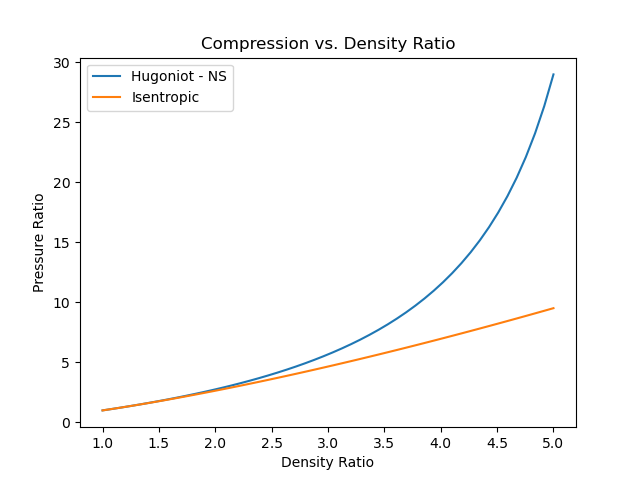
\includegraphics{../../images/problem_1/hugoniot_vs_isentropic_compression.png}
    \caption{Compression vs. density ratio -- normal shock and isentropic compression}
\end{figure}

\problempart{c}

\discussion{}

\begin{figure}[h]
    \centering
    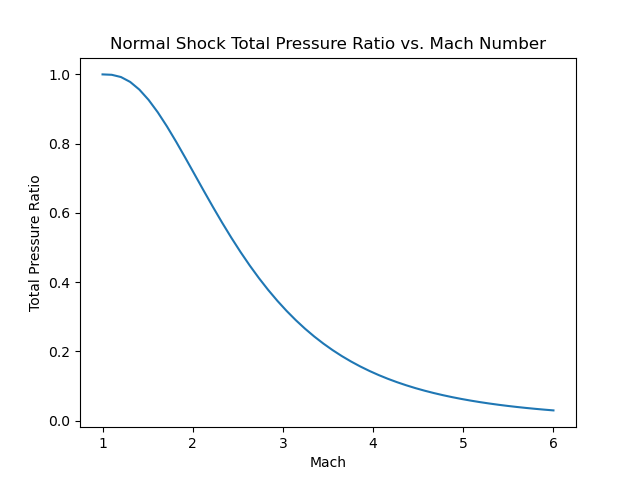
\includegraphics{../../images/problem_1/compression_efficiency_NS.png}
    \caption{Compression vs. Mach number across normal shock}
\end{figure}

\problempart{d}

\solution{}

Isentropic should be equal to 0.

\[
    s_2 - s_1 = cp \ln{\left({\frac{T_2}{T_1}}\right)} - R \ln{\left({\frac{p_2}{p_1}}\right)}
\]

\[
    \frac{T_2}{T_1} = \left({\frac{\rho_2}{\rho_1}}\right)^{\gamma-1}
\]

Across a normal shock:

\[
    s_2 - s_1 = -R \ln {\frac{p_{t,2}}{p_{t,1}}}
\]

\[
    \frac{p_2}{p_1} = 1 + \frac{2\gamma}{\gamma+1}\left(M_1^2-1\right)
\]

\[
    M_1 = \sqrt{\left({\frac{p_2}{p_1} - 1}\right)\left({\frac{\gamma+1}{2\gamma}}\right) + 1}
\]

\[
    \frac{p_{t,2}}{p_{t,1}} = big gross equation
\]

\end{document}